\documentclass[a4paper,12pt]{article}
\usepackage{cite}
\usepackage{braket}
\usepackage{amsmath}
\usepackage{graphicx}
\DeclareGraphicsExtensions{.png, .eps}
\usepackage{feynmp-auto}
\usepackage[skip=12pt]{caption}
%\usepackage{subcaption}
\captionsetup[subfloat]{captionskip=20pt}
\usepackage{xcolor}
\usepackage{lineno}
\usepackage{amssymb}
\usepackage{cancel}
\usepackage{setspace}
\usepackage{subfig}
\usepackage{slashed}
\usepackage{bm}
\usepackage[margin=1in]{geometry}
\newcommand\makebetter[1]{\textcolor{red}{\textbf{TODO:}} {#1}}
\begin{document}

\begin{center}
    \huge Search for Light Dark Matter at the LHC 
\end{center}
\begin{center}
    \large Joshua C. Hiltbrand
\end{center}
\begin{center}
    \small \today
\end{center}
\linenumbers

\section{Introduction}

    A long, outstanding problems in physics is that seemingly a majority of the
    universe is composed of non-baryonic, dark matter and dark energy. Evidence
    for this dark matter and dark energy is well established; in the discrepant
    rotation velocity curves of stars around galactic centers and the inferred
    mass through gravitational lensing observation, as well as others. Yet, the
    properties of dark matter and dark energy are not very well understood
    beyond their gravitational interactions. The particle nature of dark matter
    and its mass are still unconstrained and models with different mass ranges
    abound. One of the possible mass ranges is that of the WIMPs which would
    have a mass on the order of the $W$ or $Z$ boson and greater.  However,
    there is another mass regime of increasing interest, LDM or light dark
    matter which has a sub-GeV mass. Within this lighter mass range the model of
    interest to this paper introduces a new light force with a corresponding
    mediator, $A'$, that kinetically mixes with the standard model photon.

    A possible method of detecting light dark matter candidates under such a
    model is by explicitly producing them via a ``dark bremsstrahlung'' process.
    This accelerator-based concept for producing dark matter via dark
    bremsstrahlung could be applied to the CMS detector at the LHC. The outer
    layers of the silicon tracking system could act as a target for muons from
    the decay of a $Z$ boson to undergo a dark bremsstrahlung process. This
    paper looks to make an initial characterization of signal regions for such a
    process as applied to a Drell-Yan Monte-Carlo sample and set an expected
    background limit.

\section{Theory}

    \subsection{A Vector Portal}

        A hypothesis that is upheld in many dark matter theories is that dark
        matter was thermally created in the early, hot universe and that it was
        in thermal equilibrium with all other matter.  Dark matter particle and
        antiparticle pairs were constantly annihilating and being created in the
        thermal bath and eventually the temperature of the universe decreased enough
        that creation was no longer viable; however, the dark matter continued
        to annihilate. Then as the expansion rate of the universe exceeded the
        annihilation rate of the dark matter particles, a relic density was
        ``frozen out'' and is what we observe today; the thermal relic. This
        thermal origin constrains the possible mass range for dark matter from
        10 keV to 10 TeV. The thermal relic density that is observed today in
        turn implies a minimum coupling and cross section for annihilation of
        the dark matter particles $\sigma v \approx 3 \times 10^{-26}
        \text{cm}^3/s$. For weakly interacting, massive dark matter (WIMPs) the
        annihilation rate can be entirely achieved through a weak force coupling
        alone--the WIMP miracle; but for light dark matter ($m_{\text{DM}} \lesssim \text{GeV}$)
        the weak coupling is not sufficient, LDM would have been overproduced in
        the early universe.  In order for light dark matter to have been in
        thermal equilibrium in the early universe requires the addition of new
        light forces and corresponding mediators to annihilate through
        \cite{Holdom}.

        A few portals are possible: a Higgs, lepton and vector portals
        \cite{Pospelov}. The most predictive model \cite{Gordon} of interest to
        this paper is the vector portal with a vector mediator, $A'$ a $U(1)$
        gauge boson, which kinetically mixes with the standard model photon. The
        Lagrangian addition to the Standard Model Lagrangian is then \cite{Philip} \cite{Eder}
        \begin{equation}\label{eq:1}
            \mathcal{L} = \frac{\epsilon_Y}{2}F'_{\mu \nu} B^{\mu \nu} +
            \frac{m^2_{A'}}{2}A_{\mu}' A'^{\mu} + \overline{\chi}(i\slashed{D} -
            m_{\chi})\chi
        \end{equation}
        where the dark and hypercharge field strength tensors are defined as
        \begin{equation}
            F'_{\mu \nu} = \partial_{\mu} A'_{\nu} - \partial_{\nu}
            A'_{\mu}\text{,}
            \qquad B^{\mu \nu} = \partial^{\mu} B^{\nu} - \partial^{\nu} B^{\mu}
        \end{equation}
        and the covariant derivative is given as
        \begin{equation}
            D_{\mu} \equiv \partial_{\mu} + i g_D A'_{\mu}
        \end{equation}
        and $g_D \equiv \sqrt{4\pi \alpha_D}$ is the dark matter QED coupling
        between $A'$ and the light dark matter particle $\chi$. With the
        breaking of the electroweak symmetry the hypercharge field can be
        written in the mass eigenbasis as
        \begin{equation}
            B_{\mu} = \cos \theta_W A_{\mu} - \sin \theta_W Z_{\mu}
        \end{equation}
        which lets the Lagrangian become 
        \begin{equation}
            \mathcal{L} =  - \frac{1}{4} F_{\mu \nu}' F'^{\mu \nu} +
            \frac{\epsilon}{2} F_{\mu \nu}' F^{\mu \nu} +
            \frac{m_{A'}^2}{2}A_{\mu}' A'^{\mu} + \overline{\chi}(i\slashed{D} -
            m_{\chi})\chi
        \end{equation}
        The fifth term represents the mixing between the $A'$ and $\gamma$ field
        strength tensors with the strength of the mixing given by the small
        parameter $\epsilon \equiv \epsilon_Y \cos \theta_W \ll 1$. If this fifth term
        is diagonalized the Lagrangian then becomes the following
        \begin{equation}
            \mathcal{L} =  - \frac{1}{4} F_{\mu \nu}' F'^{\mu \nu} + \epsilon e
            A'_{\mu} \sum_f Q_f \overline{f} \gamma^{\mu} f +
            \frac{m_{A'}^2}{2}A_{\mu}' A'^{\mu} + \overline{\chi}(i\slashed{D} -
            m_{\chi})\chi
        \end{equation}
        Now it is seen that the $A'$ couples to the fermion current with a
        coupling strength of $\epsilon e Q_f$.\footnote{Here we assumed
        fermionic dark matter. For bosonic dark matter the last term in
        \eqref{eq:1} becomes $|D_{\mu}\phi|^2 - m_{\phi}^2\phi^{*}\phi$.} 
        \\
        \begin{figure}[ht]
            \centering
                \subfloat[$m_{A'} < m_{\chi}$]{
                    \begin{fmffile}{kineticMixing1}
                    \begin{fmfgraph*}(150,80)

                        \fmfstraight
                        \fmfleft{i0,i1,i2}
                        \fmfright{o0,o1,o2}
                        \fmfbottom{b0,b1,b2}

                        \fmf{fermion}{i0,v1}
                        \fmf{fermion, tension=0}{v1,v2}
                        \fmf{fermion}{v2,i2}
                        \fmflabel{$\chi$}{i0}
                        \fmflabel{$\overline{\chi}$}{i2}

                        \fmf{photon}{v1,o0}
                        \fmf{photon}{v2,o2}
                        \fmflabel{$A'$}{o0}
                        \fmflabel{$A'$}{o2}

                        \fmffreeze
                        
                    \end{fmfgraph*}
                    \end{fmffile}
                }
                \qquad \qquad
                \subfloat[$m_{A'} > m_{\chi}$]{
                    \begin{fmffile}{kineticMixing2}
                    \begin{fmfgraph*}(150,80)
                        \fmfcmd{
                            path quadrant, q[], otimes;
                            quadrant = (0, 0) -- (0.5, 0) & quartercircle & (0, 0.5) -- (0, 0);
                            for i=1 upto 4: q[i] = quadrant rotated (45 + 90*i); endfor
                            otimes = q[1] & q[2] & q[3] & q[4] -- cycle;
                        }
                        \fmfwizard

                        \fmfleft{i0,i1,i2}
                        \fmfright{o0,o1,o2}
                        \fmftop{t0,t1,t2}

                        \fmflabel{$f$}{o0}
                        \fmflabel{$\overline{f}$}{o2}
                        \fmflabel{$\chi$}{i0}
                        \fmflabel{$\overline{\chi}$}{i2}

                        \fmf{fermion, tension=0.5}{i0,v1,i2}
                        \fmf{fermion, tension=0.5}{o0,v2,o2}

                        \fmf{photon,label=$A'$}{v1,vint}
                        \fmf{photon,label=$\gamma$}{vint,v2}
                        \fmfv{decor.shape=otimes,decor.filled=empty, label.angle=90, label.dist=0.4cm, label=$\bm{\epsilon}$}{vint}
                        \fmflabel{$\bm{g_D}$}{v1}
                        \fmflabel{$\bm{g}$}{v2}

                    \end{fmfgraph*}
                    \end{fmffile}
                }
            \\
            \caption{The dark sector couples to the standard model through a
            kinetic mixing between dark photons and standard model photons.
            Represented above are the two cases where the mediator mass is above
            and below the dark matter particle mass.\\}
        \end{figure}

    \subsection{Dark Bremsstrahlung}

        A way of accessing the vector portal and realizing the mixing between the
        visible photon and dark photon is through a ``dark bremsstrahlung''
        process. As shown in the right panel of the figure above, a standard
        model lepton (lepton scattering is the focus of this paper) is incident
        on an atomic nucleus target and scatters off of it through the
        interaction with a standard model photon. The ``dark'' part occurs when
        the lepton propagator radiates a massive, dark photon.  Subsequently
        this dark photon, which can be off-shell, produces a dark matter particle
        anti-particle pair.
        
        \begin{figure}[ht]
            \centering
                \begin{fmffile}{darkBrem}
                \begin{fmfgraph*}(200,100)

                    \fmfstraight
                    \fmfleft{i0,i1,i2,i3,i4,i5}
                    \fmfright{o0,o1,o2,o3,o4,o5}
                    \fmftop{t0,t1,t2,t3,t4,t5,t6,t7,t8,t9,t10}

                    \fmf{phantom}{i0,v0,o0}
                    \fmf{fermion}{f0,v2}
                    \fmf{phantom}{v2,o2}
                    \fmfforce{(0.01w,0.5h)}{f0}
                    \fmfforce{(0.25w,0.5h)}{v2}
                    \fmfforce{(0.25w,0.1h)}{v0}
                    \fmf{photon,label=$\gamma$,tension=0}{v2,v0}
                    \fmfv{decor.shape=circle,decor.filled=empty,decor.size=9thick}{v0}
                    \fmffreeze
                    \fmf{fermion}{v2,v3}
                    \fmf{photon, label=$A^{'(*)}$}{v3,v4}
                    \fmfforce{(0.45w,0.7h)}{v3}
                    \fmfforce{(0.7w,0.7h)}{v4}
                    \fmf{phantom}{v4,o3}
                    \fmf{fermion}{v3,t6}
                    \fmf{fermion}{v4,o3}
                    \fmf{fermion}{o4,v4}
                    \fmflabel{$\chi$}{o3}
                    \fmflabel{$\overline{\chi}$}{o4}
                    \fmflabel{$l$}{f0}
                    \fmflabel{$l$}{t6}

                \end{fmfgraph*}
                \end{fmffile}
            \caption{A lepton undergoes dark bremsstrahlung whereby a
            massive mediator, $A'$, is radiated and produces light dark matter
            particles. The dark photon can be off-shell.}
        \end{figure}

        Although standard model bremsstrahlung and dark bremsstrahlung are
        diagrammatically very similar, their kinematics are distinct due to $A'$
        being a massive mediator.  With a massive, radiated mediator, the kinematic
        phase-space distribution favors recoil angles for the recoiling lepton
        where the $A'$ carries away a majority of the incident energy and momentum. In
        stark contrast, the kinematic phase space of standard model bremsstrahlung
        is peaked in the forward direction for the recoiling lepton; all scattering
        angles are small and the photon does not typically carry a majority of the
        incident lepton energy.

\section{The CMS Detector}

    The \textbf{C}ompact \textbf{M}uon \textbf{S}olenoid is a 15 m by 15 m by 21
    m, 12,500 ton particle detector operating at the \textbf{L}arge \textbf{H}adron
    \textbf{C}ollider on the border of France and Switzerland. The LHC itself is a
    proton-proton collider consisting of several synchrotron rings, currently
    operating at a CM energy of $\sqrt{s} = 13$ TeV. The CMS experiment intends to 
    make definitive measurements of various particle properties while also making
    discoveries of new physics. A comprehensive overview of the CMS detector can be
    found in \cite{CMSTDR}.

    A critical component of the CMS detector is the superconducting magnet that
    directly immerses a majority of the subdetectors in a 3.8 T magnetic field.
    The aluminum solenoid can support a current up to 20 kA and an iron yoke
    completes the device to guide the flux-return.  The magnetic field bends the
    trajectories of charged particles allowing their momentum to be measured via
    the curvature of their traversed path. To be able to determine the charge of
    a muon with a momentum of 1 TeV, the bending must be sufficient to allow for
    10\% momentum resolution. 

    The inner most subdetector is the silicon tracker which provides coverage
    for $|\eta| < 2.5$.\footnote{Pseudorapidity, denoted by $\eta$, is defined
    as $\eta \equiv -\ln \left(\frac{\tan\,\theta}{2}\right)$ where $\theta$ is
    the polar angle assuming a $z$-axis along the beamline} The innermost
    subsystem of the silicon tracker is the pixel tracker. These pixels are
    closest to the interaction point and thus endure the highest flux of
    particles thereby necessitating the use of small sensors with dimensions 100
    $\times$ 150 $\mu$m. The pixel tracker provides excellent resolution in $r$
    and $\phi$ allowing for precise measurements of momentum to be calculated
    from reconstructed tracks. A muon with a transverse momentum of 100 GeV can
    be measured with less than 10\% resolution. 

    \begin{figure}[ht]
        \begin{center}
            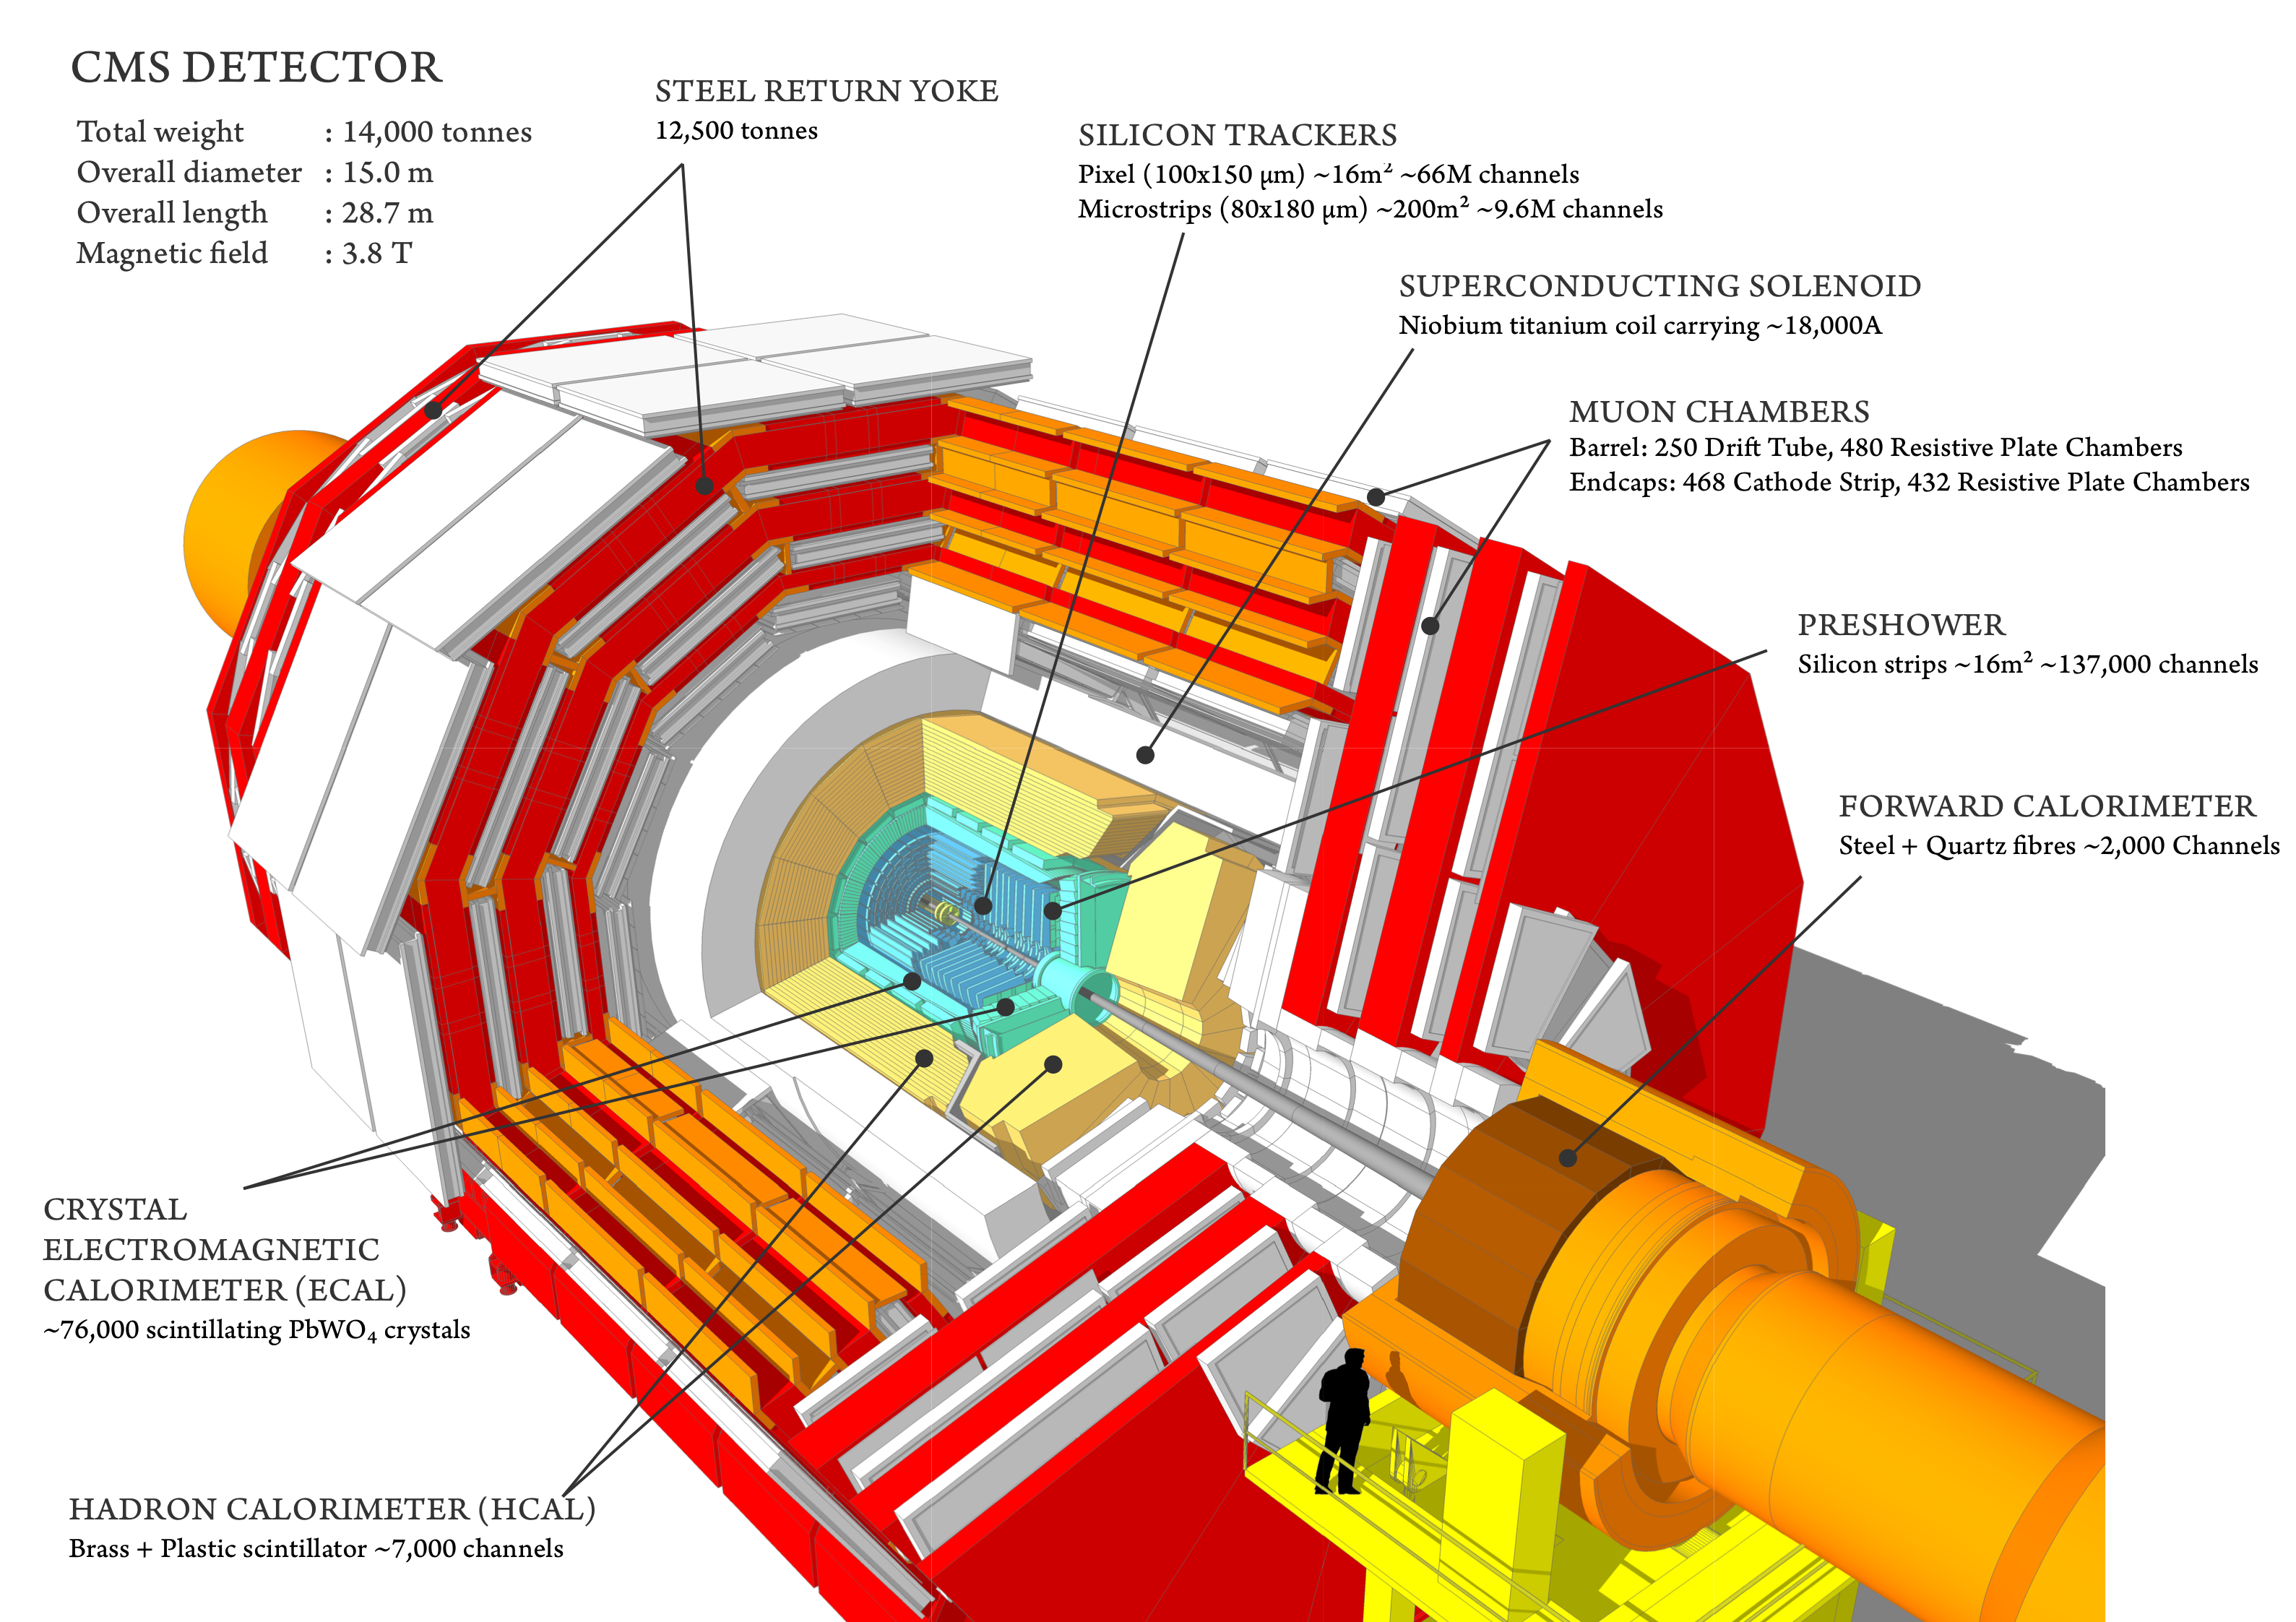
\includegraphics[width=0.9\linewidth]{Figures/CMS_Detector_Cutaway.png}
        \end{center}
        \caption{A three-quarter cutaway view of the CMS detector showing the
        concentricity of the various subdetectors and other
        components making up the device.\cite{CMSCutaway}}
        \label{fig:cms}
    \end{figure}
    
    The outer subsystem of the silicon tracker is the strip tracker. The strips
    are only granular in one dimension and therefore this is the only dimension
    that can be natively measured with reasonable resolution. To regain
    measurement in the second dimension the inner two layers have strips that
    are skewed by an angle of 100 mrad with respect to one another allowing
    reconstruction of the second dimension. This stereo configuration has a
    resolution in $z$ of 52 $\mu$m. 
    
    The next subdetector beyond the silicon tracker is the electromagnetic
    calorimeter (ECal). The ECal is composed of 61,200 (14,648) lead tungstate
    crystals placed into barrel (endcap) modules. Lead tungstate has a short
    radiation length and quick response time while still being relatively
    radiation hard and is the ideal scintillator for the ECal. It is the ECal's
    responsibility to make energy measurements of particles primarily through
    electromagnetic interactions while also providing general positional
    information. For energies above 20 GeV, the ECal exhibits an energy
    resolution below 1\%.

    Surrounding the ECal is the hadronic calorimeter or HCal. The HCal
    compliments the ECal in measuring energy of particles, particularly neutrons
    and other hadrons that are likely to escape the ECal before depositing all
    of their energy. The composition of HCal is alternating layers of brass
    absorber (chosen due its non-magnetic properties) and plastic scintillator
    for sampling the particles energy. Like the ECal the HCal has a barrel and
    endcap configuration.

    Finally, encapsulating the tracker, calorimeters and solenoid magnet and
    embedded in the flux-return yoke is the muon system. It is comprised of
    three subsystems: drift tube chambers, cathode strip chambers and resistive
    plate chambers. While the resistive plate chambers can be found in the
    barrel and endcap regions the drift tube chambers are relegated solely to
    the barrel and the cathode strip chambers to the endcap. As the systems name
    suggests, the muon system identifies muons and via the curvature of their
    reconstructed path measures their momentum and charge sign. When combined
    with the silicon tracker, the full system exhibits momentum resolution of
    $1\% - 10\%$ with the transition happening around $p_T \approx 100
    \text{GeV}$.

    The LHC's bunch crossing rate of 40 MHz simply yields too many interactions
    per second to all be written to storage, thus CMS employs triggers to reduce
    this rate. The Level-1 (L1) trigger takes in the 40 MHz and can reduce this
    down to around 100 kHz by only considering events with reconstructed objects
    like photons, leptons or jets with transverse momentum requirements. This
    reduced rate of event information is then passed into the high-level trigger
    (HLT) which uses more sophisticated software algorithms to get the rate down
    to around 100 Hz. 100 Hz is the final rate at which event data is written
    to storage.

\section{Event Selection}

    \subsection{Signal Definition}

        The signal physics process being considered is a muon undergoing
        dark bremsstrahlung in one of the outer layers of the silicon tracker
        whereby a dark photon is radiated and decays to dark matter. When the
        muon makes this interaction this will incur a discontinuity in the
        moun's full path as it traverses the detector. Since the muon is
        deflected, its track will be subject to missing hits in the last layers
        of the silicon tracker. Due to the first derivative discontinuity in the
        muon's path and its track missing hits, it will likely not be
        reconstructed as a ``global'' muon (information spanning the silicon
        tracker to the muon chamber) and will be lost. A candidate signal event
        has a track in the silicon tracker which is missing outer hits and has
        no corresponding global muon to match to it. In the direction of the
        track before the interaction point, there should also be little
        activity in the calorimeters as the dark matter takes incident momentum
        energy away undetected.

    \subsection{Basic Acceptance}

        The first selection pass made on the events is a basic acceptance
        selection. Events are selected by the single muon trigger which requires
        there to be at least one reconstructed muon in the event with a
        transverse momentum of $p_{T} \gtrsim 25$~GeV.  Following this selection
        by the trigger a recommended variety of cuts are applied to the
        muons. A definite requirement of $p_{T} > 26$~GeV is applied
        along with demanding $|\eta| < 2.1$. The muons are also
        required to meet a tight ID requirement which demands a high-quality
        reconstructed track and a global track fit with a $\chi^2$ fit
        requirement. Similarly, a simple acceptance selection is also applied to
        the tracks in an event.  Here we also require $p_{T} > 26$~GeV and
        $|\eta| < 2.1$. The pseudorapidity requirements ensure that the muons
        and tracks are within good acceptance of the inner tracking system.
        Lastly, all muon-track pairs must be within a standard invariant mass
        range around the $Z$ boson. We call for the invariant mass to be in the
        range $60 < m_{\mu + \text{track}} < 120$~GeV.

    \subsection{Quality Selection}

        \begin{figure}[ht]
            \begin{center}
                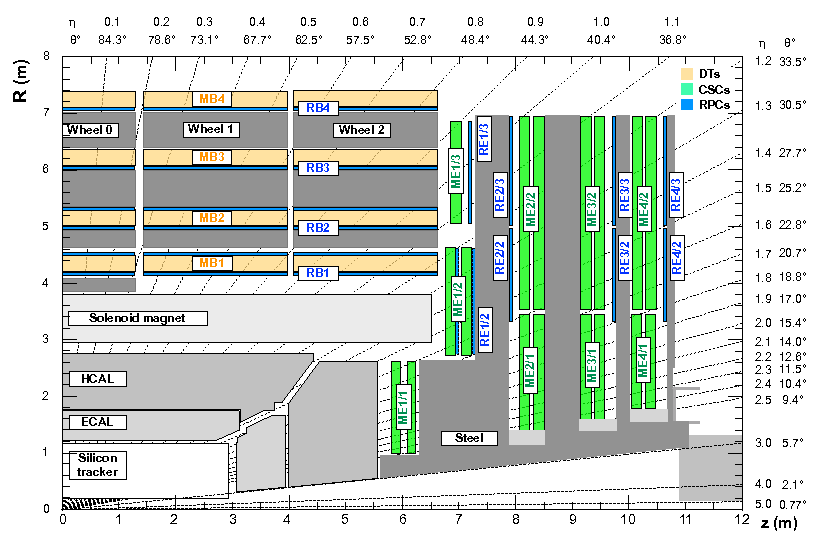
\includegraphics[scale=0.5]{Figures/CMS_rz_Cutaway.png}
            \end{center}
            \caption{An $r-z$ plane view of the CMS detector\cite{Abbiendi} allowing the
            various gaps between the calorimeters and muon chamber to be seen in
            reference to their $\eta$. Regions $0.15 < |\eta| < 0.65$, $1.42 <
            |\eta| < 1.65$ and $1.55 < |\eta| < 1.85$ are excluded.}
            \label{fig:cms_rz}
        \end{figure}

        The next level of selection applied to the events that pass the basic
        acceptance selection is a quality selection. All tracks are subject to
        an isolation condition: the sum of all the other transverse momentum
        within an angular separation of $\Delta R < 0.3$ of the track must be
        less than $10$\% of said track's $p_{T}$.\footnote{$\Delta R$ is the
        total angular separation between two objects in $\eta$-$\phi$ space and
        is defined as $\Delta R \equiv \sqrt{(\eta_1 - \eta_2)^2 + (\phi_1 -
        \phi_2)^2}$} In addition, the tracks in each event are subjected to a
        $\chi^{2}$ requirement for their respective track fits. We veto for
        $\chi^{2} > 60$ and also for $\chi^{2} < 4$. Finally, the track's number
        of hits combined with its number of missing hits must be greater than or
        equal to 12. This gets rid of tracks with a low number of hits and large
        $d_z$ but a $\chi^2$ value that passes the veto above.

        \begin{figure}[ht]%
            \centering
            \subfloat[$\chi^2$ of track fit]{{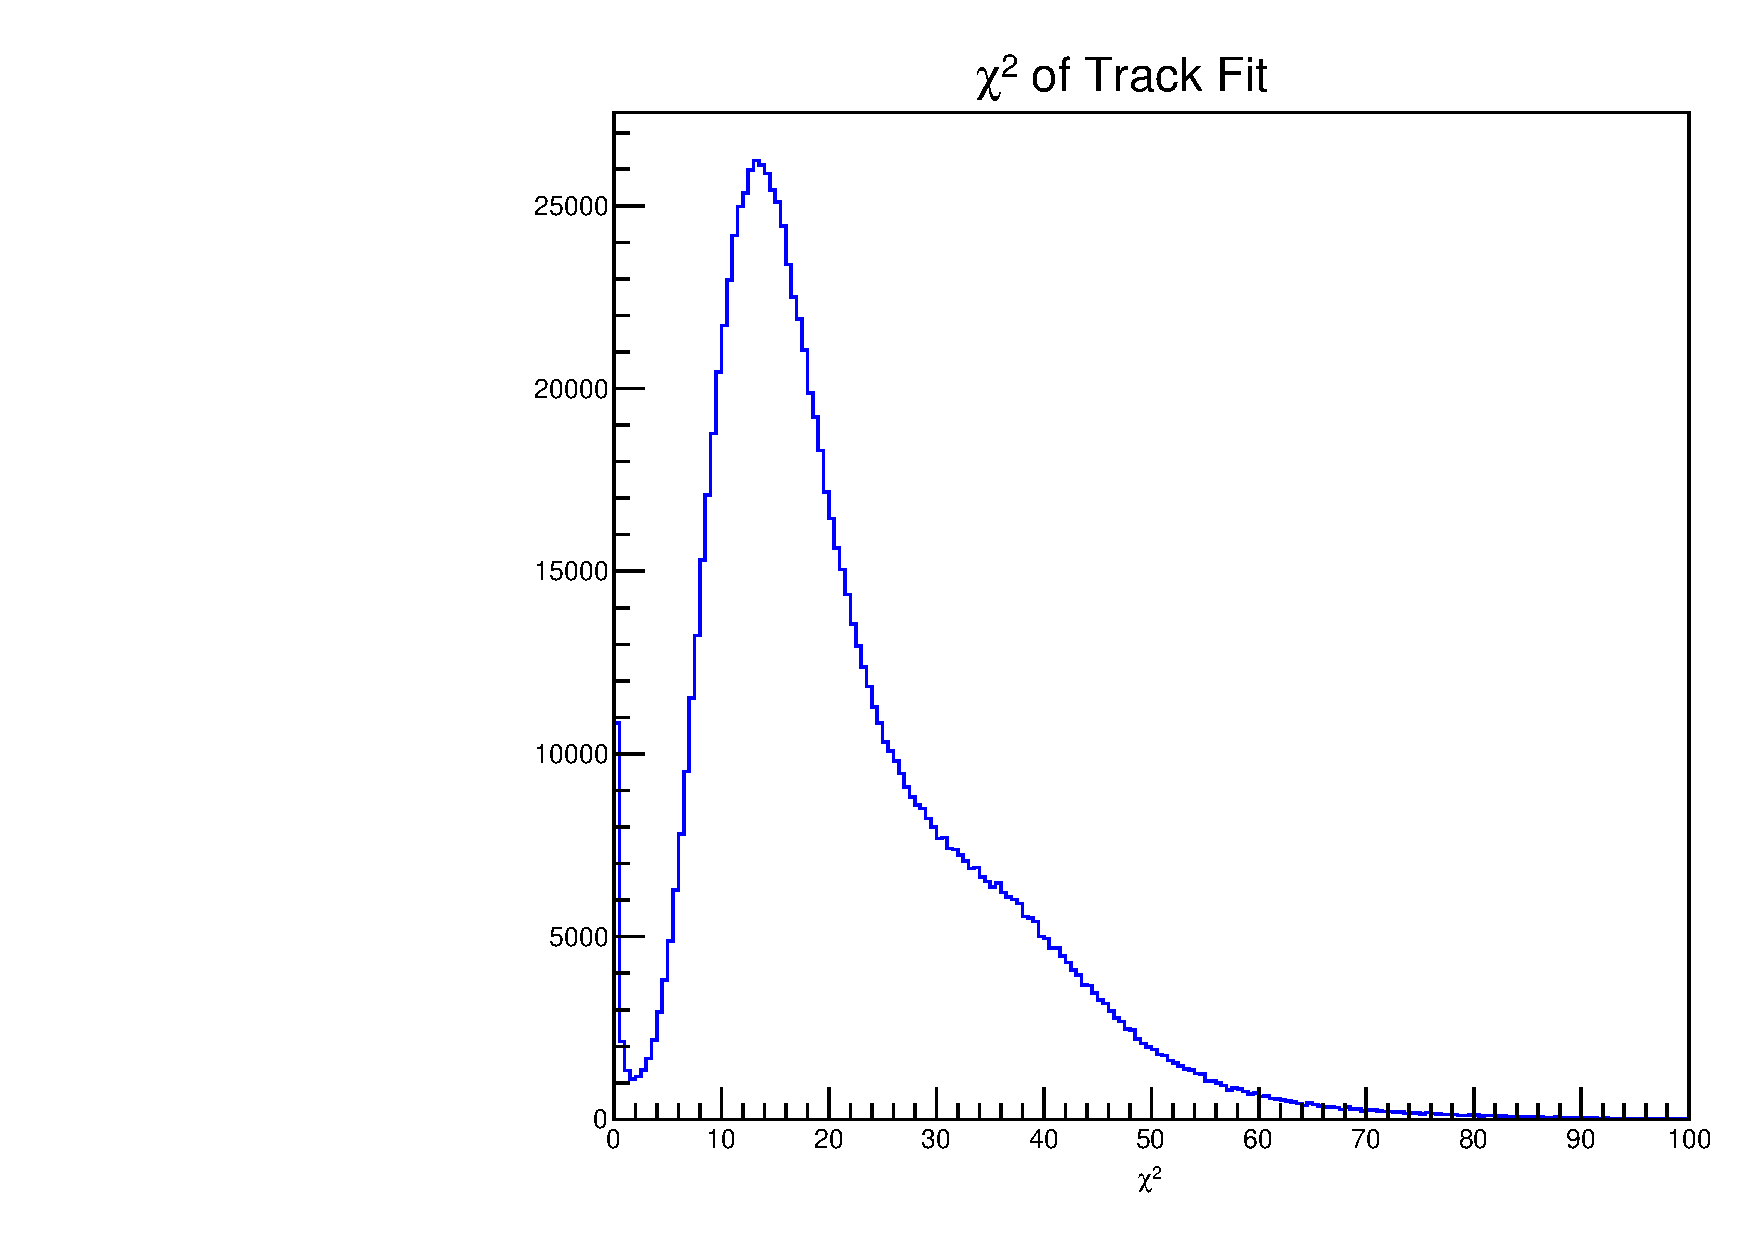
\includegraphics[width=0.45\textwidth]{Figures/acceptSelection_trkfitChi2.pdf} }}%
            \subfloat[Track $d_z$]{{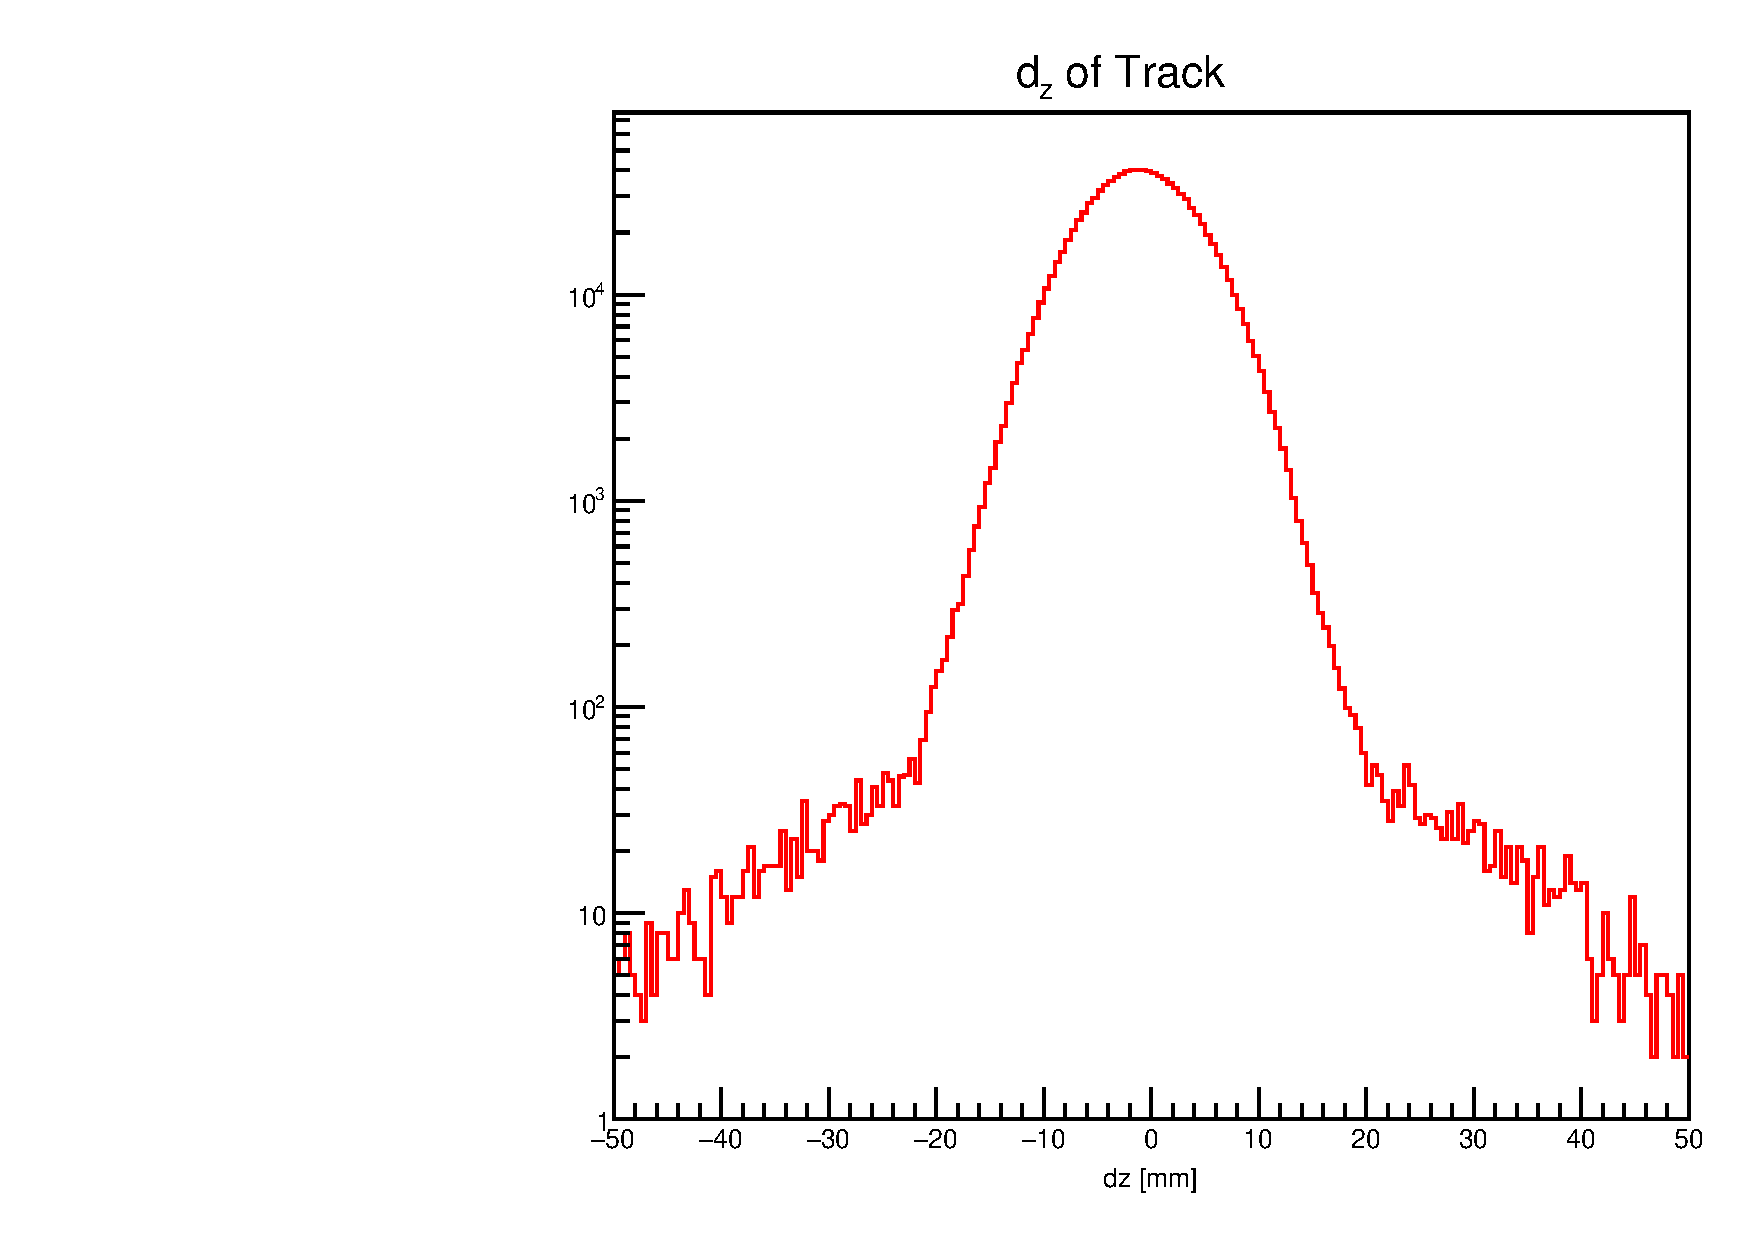
\includegraphics[width=0.45\textwidth]{Figures/acceptSelection_trkDZ.pdf} }}%
            \caption{On the left is the distribution of $\chi^2$ for the fit of
            the tracks in an event. Extremely small $\chi^2$ values corresponds
            to fits with very large errors and the corresponding tracks are
            rejected. In the right panel is the $d_z$ of the tracks. The
            non-Gaussian tails are eliminated by putting a requirement on the
            number of tracker hits plus missing hits. All events have gone
            through a basic acceptance.}
            \label{fig:chi2}
        \end{figure}

        The second part of the quality selection takes into account the detector
        geometry. The silicon tracking subdetector and muon system are not
        continuous objects, they are pieced together and therefore there are
        gaps where active sections meet. If muons and associated tracks fall
        with these regions they can lose hits and possibly get lost. These
        effects can result in tracks which appear to be missing hits and fail to
        match a muon to a track; thereby faking the signal process. To help
        curtail these possibilities from happening three regions in $\eta$-space
        are vetoed for all tracks and muons. One such region is where the endcap
        and barrel portions of the ECal and HCal meet and form a gap which
        occurs from $1.42 < |\eta| < 1.65$. A second region is at low $|\eta|$
        where there is a gap between the zeroth and first wheel of the muon
        chambers. Based on the location and orientation of this gap with respect
        to the interaction point, muons at $0.15 < |\eta| < 0.35$ see this gap
        as an extended amount of dead space thus this region is vetoed for
        inefficiency.  Finally, the region $1.55 < |\eta| < 1.85$ is vetoed due
        to gaps in the muon chamber layers that all line up and the first layer
        of CSCs being discontinuous in $z$.

    \subsection{Signal Selection}

        At this point we have a subset of events that contain a well-isolated,
        and well-fit track and we now make final selections to define a signal
        event.  In an event we now require there to be exactly one track that
        does not match to a muon. The matching criteria between a muon and a
        track is defined by the $\Delta R < 0.002$ between them. Of the events
        that pass this selection, they are then required to have low energy
        deposition in a cone of $\Delta R < 0.3$ in the direction of the
        candidate track. Specifically in the HCal and ECal there should be no
        more than 3~GeV in each calorimeter. On average a muon deposits 2~GeV in
        the HCal and it is expected that the muon will fall within a cone of
        $\Delta R < 0.3$.  Finally we select for tracks with missing hits in the
        outer silicon tracker.

\section{Results}

    After applying the full signal selection to the Drell-Yan to leptons Monte
    Carlo sample we obtain the following cutflow tables where the signal track
    is missing 1, 2 and 3 hits in the tracker.

    \makebetter{STILL NOT FINAL TABLE}

    \begin{table}[htbp] 
    \begin{center} 
    \begin{tabular}{ll}
    $\mathrm{L} = 2.613\,\mathrm{fb}^{-1}$                                                                                                                                                                                                     & \multicolumn{1}{r}{Event yield}   \\ 
    \hline 
    Pre-skimmed, single muon events           & 1557127 $\pm$ 1250.0              \\ 
    \\
    Basic Acceptance                          & 793874 $\pm$ 891.0                \\
    Quality Selection                         & 516670 $\pm$ 719.0                \\
    Signal Selection                          & 11250 $\pm$ 106.0                 \\
    \\
    $\geq$ 1 tracks with 1 missing hit        & 313 $\pm$ 17.7                    \\ 
    $\geq$ 1 tracks with 2 missing hit        & 11 $\pm$ 3.32                    \\ 
    $\geq$ 1 tracks with 3 missing hit        & 6 $\pm$ 2.45                    \\ 

    \hline 
    \end{tabular} 
    \end{center} 
    \caption{An example cutflow table with the three major acceptance and
    selection categories and the individual missing hits requirements. Note that
    the 1, 2 and 3 missing hits are not cumulative of one another, they are each 
    exclusive subsets of the signal selection.}
    \end{table} 

\section{Future Considerations}

    It is clear that the sophistication of this search can be expanded in a few
    ways. It would be useful to have a background Monte Carlo sample that
    contains not just global muons, but muons reconstructed in the muon chambers
    only and muons reconstructed in the silicon tracker only. With this
    additional information we can try and match up tracker muon and chamber muon
    tracks to be able to identify a discontinuity associated with an interaction
    of a single muon. This information can then be checked against calorimeter
    activity to get a better handle on the muon's interaction.

    A second relevant extension is to use the kinematics of a dark
    bremsstrahlung interaction due to a muon to create a signal sample to run on
    that would allow us to refine cuts in the simple signal event selection.
    With a deep understanding of the kinematics for a $\mathcal{O}
    (45\,\text{GeV})$ muon undergoing dark bremsstrahlung the various cuts could
    be made more powerful at rejecting background while still 
    preserving signal. Then we can know how significant our reduced background
    really is compared signal yield.

\section{Conclusion}

    The non-gravitational nature of dark matter is a pressing problem in physics
    today. The prospect of sub-GeV, thermal dark matter is one of many proposed
    theories for dark matter. In this paper we have made a preliminary
    quantification of the background for a light dark matter yielding process
    occurring at the LHC. With our basic acceptance, quality selection and
    final signal selection we expect a background of $6 \pm 2.45$ events when
    requiring three missing hits.

\bibliography{JCH_Oral_Paper}{}
\bibliographystyle{plain}

\end{document}
